\section{Introduction}

The behaviour of the circuit shown below in Figure \ref{fig:shematic} shall be modelled and analysed. The differential equations for the system must be established and included into a simulink model.

\begin{figure}[H]
		\centering
		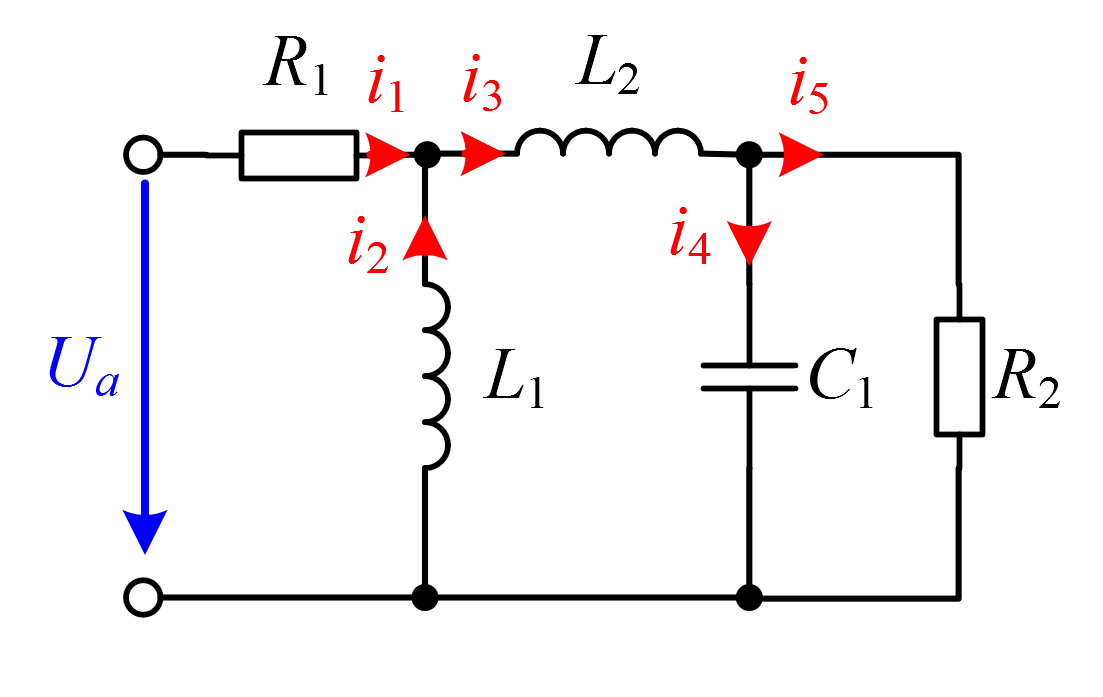
\includegraphics[width=0.7\textwidth]{figures/shematic.png}
		\caption{Schematic of the electrical system}
		\label{fig:shematic}
\end{figure}

\section{Circuit analysis}
Firstly, we'll be looking at node 1. According to Kirchoff's current law we get
\begin{equation} 
i_1+i_2-i_3=0
\end{equation}
which can be expressed as
\begin{equation}
\frac{U_{R1}}{R_1}+\frac{1}{L_1}\int U_{L1} dt -\frac{1}{L_2}\int U_{L2} dt=0
\end{equation}
Using KVL the equation can be rearranged to
\begin{equation}
\frac{U_a+U_{L1}}{R_1}+\frac{1}{L_1}\int U_{L1} dt-\frac{1}{L_2}\int (-U_3-U_{L1})dt=0
\end{equation}
Looking at the second node we get
\begin{equation}
i_3-i_4-i_5=0
\end{equation}
which again can be expressed as
\begin{equation}
\frac{1}{L_2}\int U_{L2} dt-C\frac{U_3}{dt}-\frac{U_3}{R_2}=0
\end{equation}
\begin{equation}
\frac{1}{L_2}\int (-U_3-U_{L1})dt-C\frac{U_3}{dt}-\frac{U_3}{R_2}=0 
\end{equation}
Rearranging the equations we get
\begin{equation}\label{eq:a}
\frac{U_{L1}}{R_1}=\frac{1}{L_2}\int (-U_3-U_{L1})dt-\frac{1}{L1}\int U_{L1}dt-\frac{U_a}{R_1}
\end{equation}
\begin{equation}\label{eq:b}
\frac{dU_3}{dt}C=\frac{1}{L2}\int(-U_3-U_{L1}) dt-\frac{U_3}{R_2}
\end{equation}

\section{Modelling in Simulink}
Equation \ref{eq:a} and \ref{eq:b} are only dependent on each other and $U_3$. Since $U_3$ will be given as an input, the differential equations can now be entered into simulink.
\begin{figure}[H]
		\centering
		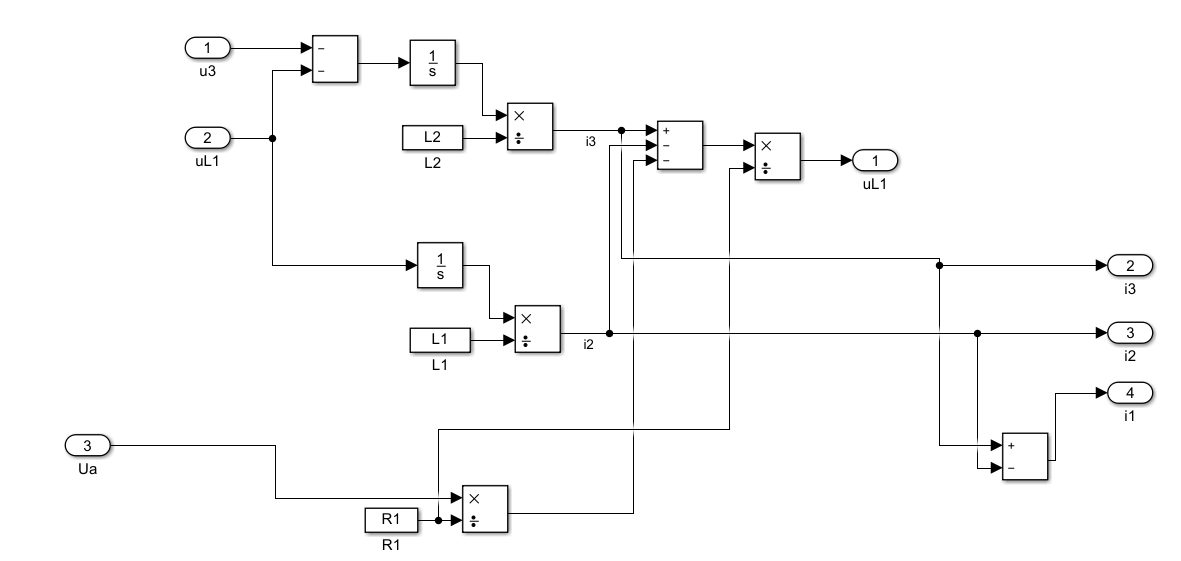
\includegraphics[width=0.7\textwidth]{figures/equation1.png}
		\caption{Implementation of equation \ref{eq:a}}
		\label{fig:equation1}
\end{figure}
\begin{figure}[H]
		\centering
		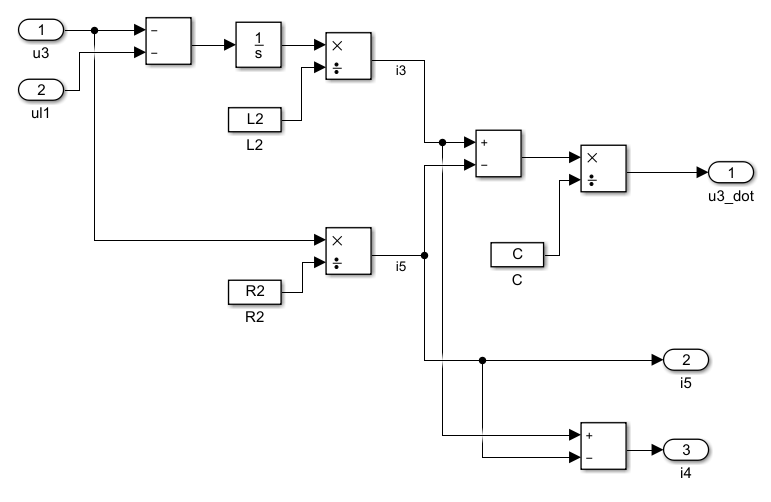
\includegraphics[width=0.7\textwidth]{figures/equation2.png}
		\caption{Implementation of equation \ref{eq:b}}
		\label{fig:equation2}
\end{figure}
In order to obtain a clearer overall model, the equations were included into subsystems. which then got connected to one another. Only basic arithmetic blocks were used. To verify the correctness of the model a constant input voltage was applied and the results were inspected. 
\begin{figure}[H]
		\centering
		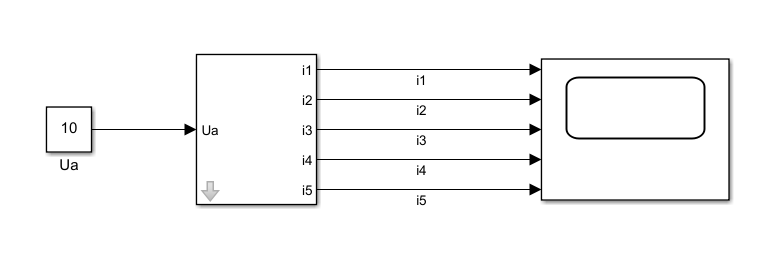
\includegraphics[width=0.7\textwidth]{figures/testsetup.png}
		\caption{Test setup of the model}
		\label{fig:testsetup}
\end{figure}
\begin{figure}[H]
		\centering
		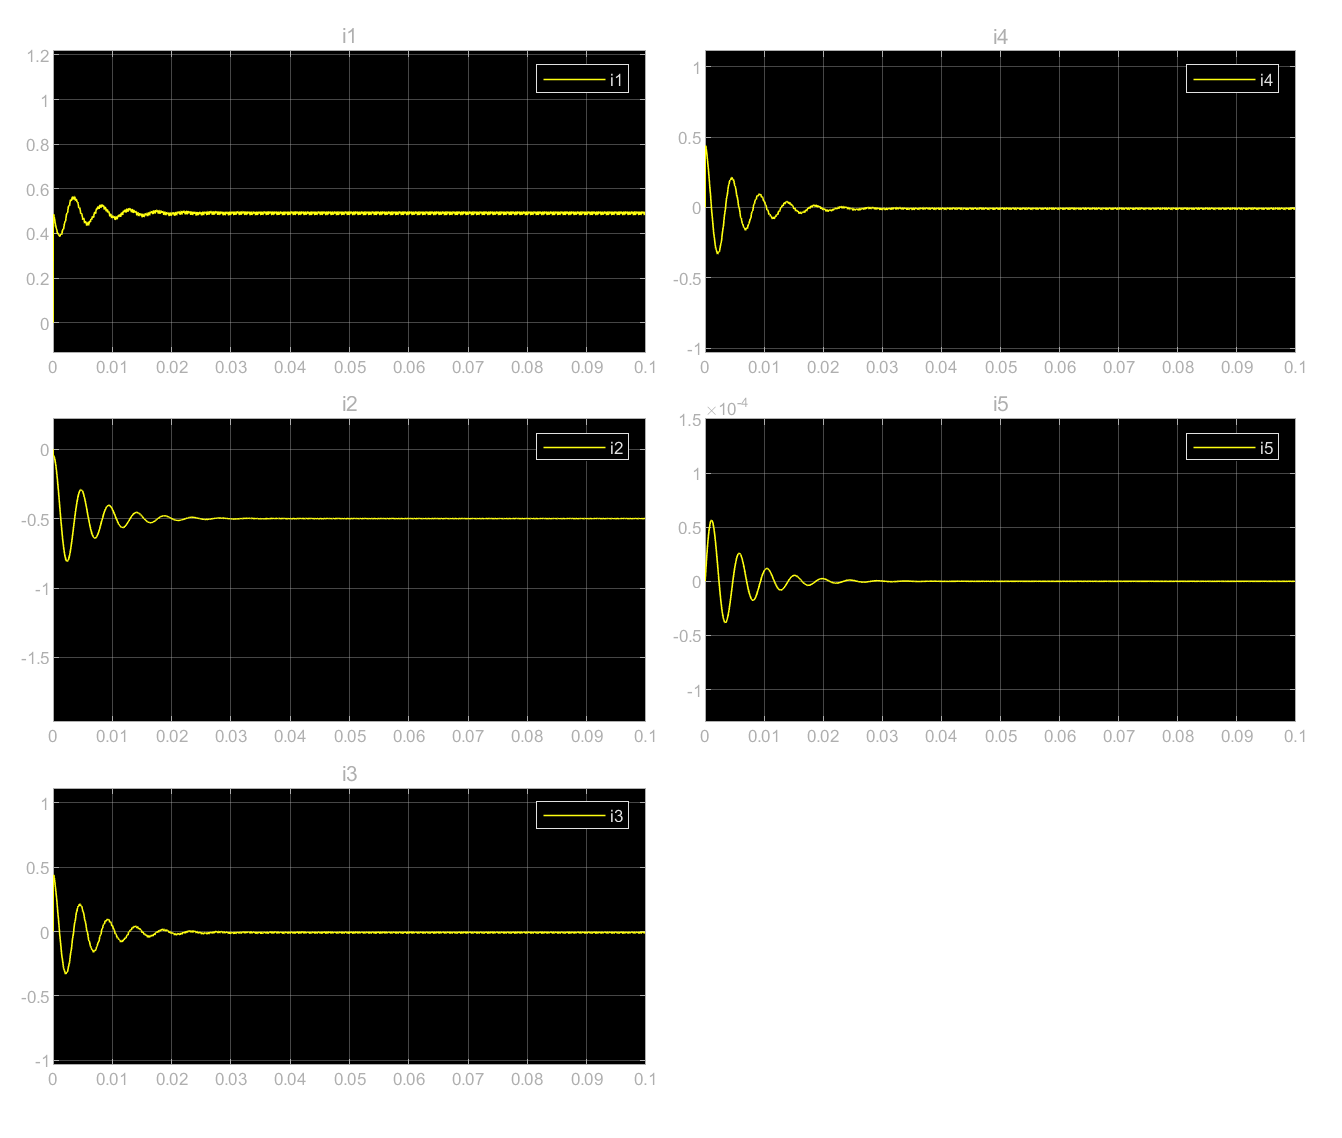
\includegraphics[width=0.7\textwidth]{figures/results.eps}
		\caption{Results of the simulation}
		\label{fig:results}
	\end{figure}
After close inspection of the results the conclusion can be drawn that the modell seems to be behaving the way it should. During the first initial timesteps there is some current $i_4$ flowing into the capacitor $C$. The inductance $L_1$ doesn't allow sudden changes in current and thus it takes some time for the current to start flowing through it. Once it has started, however, the resistance becomes very low and it almost acts like a short circuit reducing all other currents and making $i_1$ almost identical to $i_2$.
